\vspace{1cm}
\fancyhead[C]{\normalsize\textbf{$\qquad$ Teil I: Offene Aufgaben}}
\renewcommand{\labelenumi}{\theenumi.}
\section*{Aufgabe 1 (40 Punkte)}
\vspace{0.4cm}
\subsection*{\aufgabe{a}{10}}
Ein Monopolist stellt zwei Güter her.
In Abhängigkeit von den Preisen $ p_1 $ und $ p_2 $ je Mengeneinheit von Gut $ 1 $ bzw. Gut $ 2 $ lautet die
\begin{align*}
	&\textrm{Absatzmenge für Gut $ 1 $:} \quad 
	x = 30 - 3 p_1 + 2 p_2\\
	&\textrm{Absatzmenge für Gut $ 2 $:} \quad
	y = 20 + p_1 - p_2.
\end{align*}
\begin{enumerate}
	\item[\textbf{(a1)}]
	Stellen Sie den Gesamtumsatz $ U(x,y) $ nur durch $ x $ und $ y  $ dar.
	\item[\textbf{(a2)}] 
	Die Produktionskosten lauten
	\begin{align*}
		K(x,y) = x^2 + xy + y^2.
	\end{align*}
	Bei welchen Produktionsmengen $ x^\ast  $ und $ y^\ast $ wird der Reingewinn $ G(x,y) $ maximal?\\
	Wie gross ist der maximale Reingewinn?
\end{enumerate}
\ \\

\textbf{Lösung:}
\begin{mdframed}
\underline{\textbf{Vorgehensweise:}}
\renewcommand{\labelenumi}{\theenumi.}
\begin{enumerate}
\item[\textbf{(a1)}] 
\begin{enumerate}
	\item[1.] Stelle die Preise in Abhängigkeit der Absatzmengen dar.
	\item[2.] Bestimme den Gesamtumsatz in Abhängigkeit von $ x $ und $ y $.
\end{enumerate} 
\item[\textbf{(a2)}] Bestimme den Reingewinn und dessen Maximum
\end{enumerate}
\end{mdframed}
\underline{\textbf{(a1)} 1. Stelle die Preise in Abhängigkeit der Absatzmengen dar}\\
Der Gesamtumsatz ist gegeben durch
\begin{align*}
	U(x,y) = x p_1 + y p_2.
\end{align*}
Die Absatzmengen $ x $ und $ y $ sind lineare Funktionen in $ p_1 $ und $ p_2 $. Deswegen lassen sich die Preise $ p_1 $ und $ p_2 $ als Funktionen in Abhängigkeit von $ x $ und $ y $ darstellen.
Die Absatzmengen sind gegeben durch
\begin{align*}
	\textrm{(I)}&	x = 30 - 3 p_1 + 2 p_2\\
	\textrm{(II)}&  y = 20 + p_1 - p_2 .
\end{align*}
Die Addition des zweifachen der zweiten Gleichung auf die erste Gleichung ergibt:
\begin{align*}
	x + 2y = 70 - p_1
	\ \Leftrightarrow \ 
	p_1 = 70 - x - 2y.
\end{align*}
Durch Einsetzen in Gleichung (II) erhalten wir:
\begin{align*}
	y = 20 + 70 - x - 2y - p_2 
	\ \Leftrightarrow \
	p_2 = 90 -x - 3y.
\end{align*}
Damit haben wir für die Preise $ p_1 $ und $ p_2 $ die Darstellungen:
\begin{align*}
	p_1 &= 70 - x - 2y\\
	p_2 &= 90 -x - 3y.
\end{align*}
\ \\
\underline{2. Bestimme den Gesamtumsatz in Abhängigkeit von $ x $ und $ y $}\\
Mit den Preisen erhalten wir für den Gesamtumsatz
\begin{align*}
	U(x,y) = 
	x p_1 + y p_2 = 
	x (70 - x - 2y) + y (90 -x - 3y)
	=
	70x + 90 y- x^2 - 3 xy - 3 y^2.
\end{align*} 
Damit ist der Gesamtumsatz nur durch $ x $ und $ y $ dargestellt.\\
\\
\underline{\textbf{(a2)} Bestimme den Reingewinn und dessen Maximum}\\
Der Reingewinn ist gegeben als 
\begin{align*}
	G(x,y) &= U(x,y) - K(x,y) = 70x + 90 y- x^2 - 3 xy - 3 y^2 - (x^2 + xy + y^2 )\\
	&=
	70x + 90 y- 2x^2 -4 xy- 4 y^2.
\end{align*}
Die notwendige Bedingung für Extrem-und Sattelpunkte $ (x_0,y_0) $ von $ G $ ist
\begin{align*}
	G_x(x_0,y_0) =0 \\
	G_y(x_0,y_0) =0.
\end{align*}
Die partiellen Ableitungen sind:
\begin{align*}
	G_x(x,y) &= 70 - 4x - 4 y\\
	G_y(x,y) &= 90 -8y -4 x.
\end{align*}
Damit ergibt sich aus der notwendigen Bedingung das lineare Gleichungssystem
\begin{align*}
	70 - 4 x_0 - 4y_0 &= 0 \ \Leftrightarrow \ 4 x_0 + 4 y_0 = 70\\
	90 - 8 y_0 - 4 x_0 &= 0 \ \Leftrightarrow \ 4x_0 + 8y_0 = 90.
\end{align*}
Umgeschrieben in die erweiterte Koeffizientenmatrix erhalten wir mit dem Gauß-Verfahren:
\begin{align*}
	\begin{pmatrix}
		4 & 4 & \BAR &  70\\
		4 & 8 & \BAR & 90
	\end{pmatrix}
	\leadsto
	\begin{pmatrix}
		4 & 4 & \BAR &  70\\
		0 & 4 & \BAR & 20
	\end{pmatrix}
\leadsto
\begin{pmatrix}
	4 & 0 & \BAR &  50\\
	0 & 4 & \BAR & 20
\end{pmatrix}
\leadsto
\begin{pmatrix}
	1 & 0 & \BAR &  \frac{50}{4}\\
	0 & 1 & \BAR & 5
\end{pmatrix} \ \Rightarrow x_0 = \frac{50}{4}  =12.5, y_0 = 5
\end{align*}
Damit ist $ (x_0,y_0 ) = (12.5, 5) $ der einzige Kandidat für ein Maximum.\\
Für ein Maximum müssen wir noch die hinreichende Bedingung 
\begin{align*}
	&G_{xx}(x_0,y_0) < 0 \\
	&G_{yy}(x_0,y_0) < 0\\
	&\Delta(x,y) := G_{xx}(x_0,y_0)G_{yy}(x_0,y_0)-(G_{xy}(x_0,y_0))^2 > 0
\end{align*}
überprüfen. Dafür bestimmen wir die partiellen Ableitungen zweiter Ordnung von $ G $:
\begin{align*}
	G_{xx}(x,y) = -4 < 0, \
	G_{yy}(x,y) = -8 < 0, \ 
	G_{xy}(x,y) = G_{yx}(x,y) = -4.
\end{align*}
Hiermit folgt
\begin{align*}
	\Delta(x,y) = G_{xx}(x_0,y_0)G_{yy}(x_0,y_0)-(G_{xy}(x_0,y_0))^2
	= (-4)\cdot(-8) - (-4)^2 = 16  >0
\end{align*}
für alle $ (x,y) \in \mathbb{R}^2 $. Insbesondere gilt dies auch für unseren Kandidaten $ (x_0,y_0) = (12.5,5) $, womit dieser ein Maximum ist. Der maximale Reingewinn ist:
\begin{align*}
	G(12.5,5) = 662.5 \ \textrm{(CHF)}.
\end{align*} 





\newpage

\subsection*{\aufgabe{b}{14}}
Je nach Konjunktur (gut, mittel, schlecht) haben drei Aktien unterschiedliche zu erwartende Auszahlungen.
\begin{table}[H]
	\centering
	%
	\begin{tabular}{|l |c |c |c|}
		\hline
		\multirow{3}{*}{Konjunktur}
		& erwartete Auszahlung	& erwartete Auszahlung & erwartete Auszahlung\\
		& pro Einheit von & pro Einheit von & pro Einheit von\\
		& Aktie 1 & Aktie 2	& Aktie 3\\
		\hline
		gut & $ 2 $  &  $ a $ &  $ 5 $ \\ 
		\hline
		mittel & $ 1 $ & $ 1 $ & $ 1 $  \\ 
		\hline
		schlecht & $ 0 $ & $ 1 $ & $ a $ \\
		\hline
	\end{tabular}%
\end{table}
Gesucht sind geeignete Kombinationen dieser Geldanlagen (Käufe, respektive Leerverkäufe), die bei guter Konjunktur die Auszahlung $ 7'000 $, bei mittlerer Konjunktur die Auszahlung $ 5'000 $ und bei schlechter Konjunktur die Auszahlung $ 1'000 $ ergeben.
\begin{enumerate}
	\item[\textbf{(b1)}]
	Bestimmen Sie ein lineares Gleichungssysteme für die benötigten Einheiten $ x_i \in \mathbb{R} $ der Anteile an Aktie $ i \in \{1,2,3\} $, die man haben muss, um bei jeder Konjunkturlage die gewünschte Auszahlung erreichen zu können.
	\item[\textbf{(b2)}] 
	Für welche Werte von $ a \in \mathbb{R} $ gibt es eine eindeutige Kombination?
	Für welche Werte von $ a \in \mathbb{R} $ gibt es keine mögliche Kombination?
	Für welche Werte von $ a \in \mathbb{R} $ gibt es unendlich viele mögliche Kombinationen?
	\item[\textbf{(b3)}]
	Berechnen Sie im Falle einer eindeutigen Lösung die Lösung $ (x_1,x_2,x_3) $ (in Abhängigkeit von $ a $).
	\item[\textbf{(b4)}]
	Beschreiben Sie die Lösungsgesamtkeit der möglichen Kombinationen, wenn es unendlich viele Lösungen gibt.
\end{enumerate}
\ \\
\textbf{Lösung:}
\begin{mdframed}
\underline{\textbf{Vorgehensweise:}}
\renewcommand{\labelenumi}{\theenumi.}
\begin{enumerate}
\item[\textbf{(b1)}] Stelle das lineare Gleichungssystem auf.
\item[\textbf{(b2)}] Verwende das Gauß-Verfahren.
\item[\textbf{(b3)}] Bestimme die eindeutige Lösung.
\item[\textbf{(b4)}] Bestimme den unendlichen Lösungsraum.
\end{enumerate}
\end{mdframed}

\underline{\textbf{(b1)} Stelle das lineare Gleichungssystem auf}\\
Die Auszahlungen ergeben für gute, mittlere und schlechte Konjunktur die Linearkombination
\begin{align*}
	\underbrace{x_1}_{\textrm{Anzahl Aktie 1}}
	\underbrace{\begin{pmatrix}
		2 \\ 1 \\ 0
	\end{pmatrix}}_{\textrm{erwartete Auszahlung  Aktie 1}}
	+
	x_2 
	\begin{pmatrix}
		a \\ 1 \\ 1
	\end{pmatrix}
	+
	x_3
	\begin{pmatrix}
		5 \\ 1 \\ a
	\end{pmatrix}
	= 
	\begin{pmatrix}
		7'000\\
		5'000\\
		1'000\\
	\end{pmatrix}.
\end{align*}
Hier stellen die Zeilen absteigend die gute bis schlechte Konjunktur dar. Umgeschrieben in ein lineares Gleichungssystem erhalten wir:
\begin{align*}
	\textrm{gut:} \quad 2 x_1 + a x_2 + 5 x_3 &= 7'000\\
	\textrm{mittel:} \quad  \ x_1 + x_2 + x_3  &= 5'000\\
	\textrm{schlecht: } \quad \ \ \ x_2 + a x_3 &= 1'000.
\end{align*}
Hieraus ergibt sich die erweiterte Koeffizientenmatrix
\begin{align*}
	(A | \mathbf{b})
	=
	\begin{pmatrix}
		2 & a & 5 & \BAR & 7'000\\
		1 & 1 & 1 & \BAR & 5'000\\
		0 & 1 & a & \BAR & 1'000
	\end{pmatrix}.
\end{align*}
\ \\
\underline{\textbf{(b2)} Verwende das Gauß-Verfahren}\\
Die Anwendung des Gauß-Verfahrens ergibt:
\begin{align*}
	\begin{gmatrix}[p]
		2 & a & 5 & \BAR & 7'000\\
		1 & 1 & 1 & \BAR & 5'000\\
		0 & 1 & a & \BAR & 1'000
		\rowops
		\swap{0}{1}
	\end{gmatrix}
	&\leadsto
	\begin{gmatrix}[p]
		1 & 1 & 1 & \BAR & 5'000\\
		2 & a & 5 & \BAR & 7'000\\
		0 & 1 & a & \BAR & 1'000
		\rowops
		\add[ \cdot (-2)]{0}{1}
	\end{gmatrix}
\leadsto
\begin{gmatrix}[p]
	1 & 1 & 1 & \BAR & 5'000\\
	0 & a - 2 & 3 & \BAR & -3'000\\
	0 & 1 & a & \BAR & 1'000
	\rowops
	\swap{1}{2}
\end{gmatrix}\\
&\leadsto
\begin{gmatrix}[p]
	1 & 1 & 1 & \BAR & 5'000\\
	0 & 1 & a & \BAR & 1'000\\
	0 & a - 2 & 3 & \BAR & -3'000
	\rowops
	\add[ \cdot (-1)]{1}{0}
	\add[ \cdot (-(a-2)), a \neq 2]{1}{2}
\end{gmatrix}\\
&\leadsto
\begin{gmatrix}[p]
	1 & 0 & 1-a & \BAR & 4'000\\
	0 & 1 & a & \BAR & 1'000\\
	0 & 0 & 3 -a(a-2) & \BAR & -3'000 - 1'000(a-2)
\end{gmatrix}\\
&=
\begin{gmatrix}[p]
	1 & 0 & 1-a & \BAR & 4'000\\
	0 & 1 & a & \BAR & 1'000\\
	0 & 0 & -a^2 + 2a  + 3  & \BAR & -1'000(a+1)
\end{gmatrix}
\end{align*}
Man beachte den Schritt mit $ a \neq 2 $. Für $ a = 2 $ besitzt $ A $ den vollen Rang, womit die Lösung eindeutig ist. Falls 
\begin{align*}
	-a^2 + 2a + 3 = -(a-3)(a+1) \neq 0 \ \Rightarrow a \neq 3 \wedge a\neq 1
\end{align*}
gilt $ \mathrm{rg}(A) = \mathrm{rg}(A | \mathbf{b}) = 3 $ und das System besitzt eine eindeutige Lösung $ \mathbf{x} = (x_1,x_2 ,x_3)^\top $.
Für 
\begin{align*}
	-a^2 + 2a + 3 = -(a-3)(a+1) = 0 \ \Leftrightarrow a = 3 \vee a = -1
\end{align*}
besitzt das LGS entweder unendlich viele Lösungen oder keine Lösung.\\
Dies ist abhängig von $ -1'000(a+1) = 0  $ oder $ -1'000(a+1) \neq 0 $.
Für $ a = 3  $ gilt $ \mathrm{rg}(A) = 2 < \mathrm{rg} (A | \mathrm{b}) = 3 $ und das LGS besitzt keine Lösung.
Für $ a = -1  $ gilt $ \mathrm{rg}(A)  = \mathrm{rg} (A | \mathrm{b}) = 2 $ und das LGS besitzt unendlich viele Lösungen.\\
\\
\underline{\textbf{(b3)} Bestimme die eindeutige Lösung}\\
Durch das Gauß-Verfahren haben wir die erweitere Koeffizientenmatrix wie folgt umgeformt:
\begin{align*}
\begin{gmatrix}[p]
	2 & a & 5 & \BAR & 7'000\\
	1 & 1 & 1 & \BAR & 5'000\\
	0 & 1 & a & \BAR & 1'000
\end{gmatrix}
\leadsto
\begin{gmatrix}[p]
	1 & 0 & 1-a & \BAR & 4'000\\
	0 & 1 & a & \BAR & 1'000\\
	0 & 0 & -(a-3)(a+1)  & \BAR & -1'000(a+1)
\end{gmatrix}
\end{align*}
Hieraus ergeben sich die Gleichungen
\begin{align*}
	x_1 + (1-a)x_3 &= 4'000\\
	x_2 + a x_3 &= 1'000\\
	-(a-3)(a+1) x_3 &= -1'000 (a+1). 
\end{align*}
Durch Einsetzen von $ x_3 $ lassen sich die $ x_1 $ und $ x_2 $-Koordinate bestimmen. Durch die Umformung
\begin{align*}
	-(a-3)(a+1) x_3 &= -1'000 (a+1) \ \Leftrightarrow \
	x_3 = -1'000 \frac{(a+1)}{-(a-3)(a+1)} = \frac{1'000}{a-3}
\end{align*}
folgt 
\begin{align*}
	x_1 &= 4'000 - (1-a)x_3 = 4'000- (1-a)\frac{1'000}{a-3}
	= \frac{4'000(a-3)}{a-3} - \frac{(1-a)1'000}{a-3}\\
	&= \frac{4'000(a-3) - (1-a)1'000}{a-3}
	= \frac{5'000 a - 13'000}{a-3} = 1'000 \frac{5a -13}{a-3}
\end{align*}
und 
\begin{align*}
	x_2 = 1'000 - a x_3 = \frac{1'000(a-3)}{a-3} - a \frac{1'000}{a - 3}
	=
	\frac{-3'000}{a-3} = \frac{3'000}{3-a}.
\end{align*}
Damit ist die eindeutige Lösung durch
\begin{align*}
	\mathbf{x}
	=
	1'000 
	\begin{pmatrix}
		 \frac{5a -13}{a-3}\\
		\frac{3}{3-a}\\
		\frac{1}{a-3}
	\end{pmatrix}
\end{align*}
gegeben.\\
\\
\underline{\textbf{(b4)} Bestimme den unendlichen Lösungsraum}\\
Für $ a = -1 $ ist die in (b2) bestimmte erweitere Koeffizientenmatrix gegeben durch:
\begin{align*}
	(A | \mathbf{b}) 
	= 
	\begin{gmatrix}[p]
		1 & 0 & 2 & \BAR & 4'000\\
		0 & 1 & -1 & \BAR & 1'000\\
		0 & 0 & 0  & \BAR & 0
	\end{gmatrix}
\end{align*}
Dies führt zu den Gleichungen
\begin{align*}
	x_1 + 2 x_3 &= 4'000
	\ \Leftrightarrow \ x_2 = 4'000 - 2 x_3
	\\
	x_2 - x_3 &= 1'000
	\ \Leftrightarrow \
	x_2 = 1'000 + x_3
\end{align*}
mit der frei wählbaren Variable $ t:=x_3 $. Damit ergibt sich die Lösungsmenge
\begin{align*}
	\mathcal{L}
	= \left\lbrace
	\mathbf{x} \in \mathbb{R}^3 \ : \
	\mathbf{x} = 
	\begin{pmatrix}
		x_1 \\ x_2 \\ x_3
	\end{pmatrix} 
	=
	\begin{pmatrix}
		4'000\\
		1'000\\
		0
	\end{pmatrix}
	+ t 
	\begin{pmatrix}
		-2\\
		1 \\
		1
	\end{pmatrix}
	\right\rbrace.
\end{align*}

\newpage
\subsection*{\aufgabe{c}{10}}
Für einen elliptischen Tisch mit den Halbachsen $ a > 0  $ und $ b > 0 $ ist eine flächenmässig möglichst grosse rechteckige Auflage anzufertigen, die an keiner Stelle übersteht.
\begin{enumerate}
	\item[\textbf{(c1)}]
	Welche Ausmasse (Länge und Breite) hat die rechteckige Auflage?
	\item[\textbf{(c2)}]
	Wie gross ist die maximale Fläche?
\end{enumerate}
\textit{Wichtige Bemerkung}: Eine Abklärung, ob es sich wirklich um ein Maximum handelt, wird \textbf{nicht} verlangt, weil es offensichtlich ein Maximum geben muss.
\\ \\
\textbf{Lösung:}
\begin{mdframed}
\underline{\textbf{Vorgehensweise:}}
\begin{enumerate}
\item[\textbf{(c1)}] Beschreibe die Situation und verwende die Symmetrie.
\item[\textbf{(c2)}] 
\begin{enumerate}
	\item[1.] Formuliere das Optimierungsproblem.
	\item[2.] Wende die Methode von Lagrange an. 
\end{enumerate}
\end{enumerate}
\end{mdframed}

\underline{\textbf{(c1)} Beschreibe die Situation und verwende die Symmetrie}\\
Die Situation der Aufgabenstellung lässt sich durch folgende Grafik darstellen:
\begin{center}
	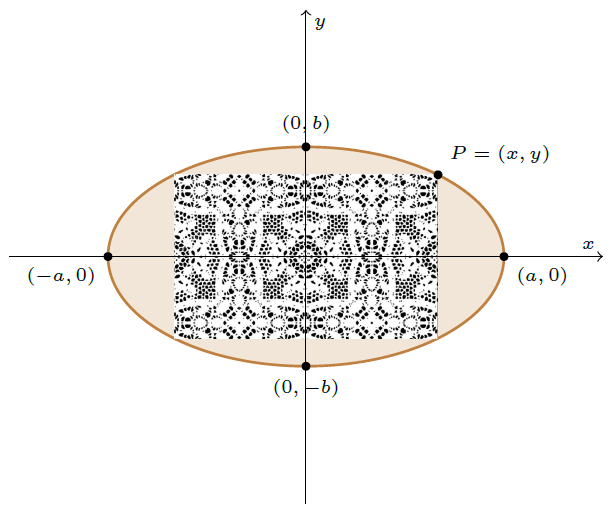
\includegraphics[width=0.6\textwidth]{pictures/aufgabe1_c}
\end{center}
Das Ziel ist es, eine größtmögliche rechteckige Auflage für einen elliptischen Tisch mit den Halbachsen $ a,b > 0  $ zu finden. Damit die Fläche maximal wird, müssen die Ecken der Auflage die Tischkante berühren.\\
Die Symmetrieeigenschaft vereinfacht uns die Berechnung der Rechtecksfläche:\\
Die Fläche $ A $ der Auflage ist genau viermal so groß wie die Fläche des Rechtecks mit einem Eckpunkt im Ursprung und einem Eckpunkt $ P = (x,y), \ x,y > 0  $ auf der Ellipse. Die Symmetrie der Ellipse liefert uns für die Auflage eine Länge von $ 2x $, eine Breite von $ 2y $ und einen Flächeninhalt von $ A = 4 xy $.\\
\\
\newpage
\underline{\textbf{(c2)} 1. Formuliere das Optimierungsproblem}\\
Alle Punkte $ P=(x,y) $ auf der Ellipse mit dem Mittelpunkt $ (0,0) $ und den Halbachsen $ a,b > 0 $ werden durch die Gleichung
\begin{align*}
	\varphi(x,y) = \frac{x^2}{a^2} + \frac{y^2}{b^2} - 1 = 0
\end{align*} 
beschrieben.
Mit unseren vorangegangen Überlegungen erhalten wir das Optimierungsproblem
\begin{align*}
	\max \limits_{x,y} A(x,y) = 4 xy
\end{align*}
unter der Nebenbedingung $ \varphi(x,y) = \frac{x^2}{a^2} + \frac{y^2}{b^2} - 1 = 0 $.\\
\\
\underline{2. Wende die Methode von Lagrange an}\\
Die Lagrange-Funktion ist durch
\begin{align*}
	L(x,y,\lambda) 
	= A(x,y) + \lambda\varphi(x,y)
	= 4xy + \lambda \left(\frac{x^2}{a^2} + \frac{y^2}{b^2} - 1\right)
\end{align*}
gegeben. Die partiellen Ableitungen dieser sind:
\begin{align*}
	\frac{\partial L}{\partial \mathrm{x}}L(x,y,\lambda)
	&= 4 y + \frac{2\lambda}{a^2} x \\
	\frac{\partial L}{\partial \mathrm{y}}L(x,y,\lambda)
	&= 4 x + \frac{2\lambda}{b^2} y \\
	\frac{\partial L}{\partial \mathrm{\lambda}}L(x,y,\lambda)
	&= \frac{x^2}{a^2} + \frac{y^2}{b^2} - 1.
\end{align*}
Hieraus ergeben sich durch Nullsetzen die Lagrange-Bedingungen:
\begin{align*}
	\textrm{(I)}& \quad 
	4 y + \frac{2\lambda}{a^2} x = 0
	\ \Leftrightarrow \ 4y = - \frac{2\lambda}{a^2} x 
	\ \Leftrightarrow \ y = -\frac{\lambda}{2a^2} x
	\\
	\textrm{(II)}& \quad 
	4 x + \frac{2\lambda}{b^2} y = 0
	\ \Leftrightarrow \
	x = - \frac{\lambda}{2 b^2} y 
	\\
	\textrm{(III)}& \quad 
	\frac{x^2}{a^2} + \frac{y^2}{b^2} - 1 = 0\\
\end{align*}
Die Gleichungen (I) und (II) sind für $ x = y = 0 $ trivialerweise erfüllt.
Der Punkt $ (0,0)  $ erfüllt jedoch die Nebenbedingung (III) nicht.
Für $ x \neq 0, y = 0$ oder $ x = 0, y \neq 0 $ gilt $ A(x,y) = 0 $.
Anschaulich kann dies nicht die maximale Fläche sein. Deswegen können wir $ x,y \neq 0 $ annehmen. Wir erhalten:
\begin{align*}
	\frac{y}{x} = \frac{-\frac{2 \lambda}{a^2} x}{- \frac{2\lambda}{b^2} y}
	= 
	\frac{b^2}{a^2} \frac{x}{y}
	\
	\Leftrightarrow \
	y^2 = \frac{b^2}{a^2} x^2
	\ \Leftrightarrow \
	\frac{y^2}{b^2} = \frac{x^2}{a^2}.
\end{align*}
Mit der Gleichung (III) folgt
\begin{align*}
	\frac{x^2}{a^2} + \frac{y^2}{b^2} - 1 = 0
	\ \Leftrightarrow \
	2 \frac{x^2}{a^2}  -1 = 0
	\ \Leftrightarrow \
	2 \frac{x^2}{a^2}   = 1
	\ \Leftrightarrow \
	\frac{x^2}{a^2} = \frac{1}{2} = \frac{y^2}{b^2}
\end{align*}
und es ergibt sich 
\begin{align*}
	\frac{x^2}{a^2} = \frac{1}{2} 
	 \ \Leftrightarrow \ 
	 x^2  = \frac{1}{2} a^2
	 \ \Leftrightarrow \
	 x = \pm \frac{1}{\sqrt{2}} a\\
	 \frac{y^2}{b^2} = \frac{1}{2} 
	 \ \Leftrightarrow \ 
	 y^2  = \frac{1}{2} b^2
	 \ \Leftrightarrow \
	 y = \pm \frac{1}{\sqrt{2}} b.
\end{align*}
Da wir die maximale Fläche suchen, ist nur die positive Lösung für $ x $ und $ y $ relevant. Für 
\begin{align*}
	x^\ast = \frac{a}{\sqrt{2}}, \quad y^\ast = \frac{b}{\sqrt{2}}
\end{align*}  
wird die Fläche $ A(x^\ast, y^\ast ) $ maximal. Die optimale Auflage hat eine Länge von $ l = 2 x^\ast = \sqrt{2} a  $ und eine Breite von $ w = 2 y^\ast = \sqrt{2} b  $.
Das führt zu der maximalen Fläche 
\begin{align*}
	A(x^\ast, y^\ast) = 2 ab.
\end{align*}
\ \\
\textbf{Alternativer Lösungsansatz}\\
Wir können das Optimierungsproblem
\begin{align*}
	\max \limits_{x,y} A(x,y) = 4 xy
\end{align*}
unter der Nebenbedingung $ \varphi(x,y) = \frac{x^2}{a^2} + \frac{y^2}{b^2} - 1 = 0$ auch durch Substitution lösen. Aufgrund der vorherigen Diskussion können wir $ x,y > 0 $ annehmen. Hieraus folgt $ A(x,y) = 4 xy > 0 $. Das führt durch
\begin{align*}
	A(x,y) = 4 xy \ \Leftrightarrow \
	\frac{1}{4} A(x,y) = xy
	\ \Leftrightarrow \
	\overline{A}(x,y) := \frac{1}{16}A(x,y) = x^2 y^2
\end{align*}
zu einem äquivalenten Optimierungsproblem. Durch Umformung der Nebenbedingung
\begin{align*}
	\frac{x^2}{a^2} + \frac{y^2}{b^2} - 1 = 0 
	\ \Leftrightarrow \
	x^2 = a^2\left(1 - \frac{y^2}{b^2} \right) = a^2 - \frac{a^2}{b^2} y^2
\end{align*}
erhalten wir durch
\begin{align*} 
	F(y) = \left(a^2 - \frac{a^2}{b^2} y^2\right) y^2
\end{align*}
eine Funktion, welche sich gut für eine eindimensionale Kurvendiskussion eignet. Der Faktor $ \frac{1}{16} $ wurde hier bewusst ignoriert, da dieser keine Auswirkung auf das Maximum hat.
\newpage
\subsection*{\aufgabe{d}{6}}
\begin{enumerate}
	\item[\textbf{(d1)}]
	Gesucht sind alle (positiven) Funktionen $ f(x) $, welche für alle $ x > 0 $ die Elastizität
	\begin{align*}
		\varepsilon_f(x) = \frac{1}{x}
	\end{align*}
	besitzen.\\
	\textit{Tipp:} Erinnern Sie sich, dass für positive Funktonen $ f(x) $ gilt:
	\begin{align*}
		\frac{d}{dx} \ln(f(x)) = \rho_f(x) 
		\ \textrm{und} \
		\varepsilon_f(x) = x \cdot \rho_f(x),
	\end{align*}
	wobei $ \rho_f $ die Wachstumsrate von $ f $ ist.
	\item[\textbf{(d2)}]
	Welche positive Funktion $ f(x) $ mit $ f(1) = 1 $ besitzt die Elastizität $ \varepsilon_f(x) = \frac{1}{x} $ für alle alle $ x >0 $.
\end{enumerate}
\ \\
\textbf{Lösung:}
\begin{mdframed}
\underline{\textbf{Vorgehensweise:}}
\begin{enumerate}
\item[\textbf{(d1)}]
\begin{enumerate}
	\item[1.] Verwende die Definition der Elastizität und der Wachstumrate.
	\item[2.] 
	Bestimme alle positiven Funktionen mit der vorgebenden Elastizität.
\end{enumerate}
\item[\textbf{(d2)}] 
Verwende die erste Teilaufgabe.
\end{enumerate}
\end{mdframed}

\underline{\textbf{(d1)} 1. Verwende die Definition der Elastizität und der Wachstumrate}\\
Die Elastizität von $ f $ in $ x $ ist gegeben durch
\begin{align*}
	\varepsilon_f(x) := x \cdot \underbrace{\frac{f^\prime(x)}{f(x)}}_{\rho_f(x)},
\end{align*} 
wobei $ \rho_f(x) $ die Wachsstumsrate von $ f $ ist. 
Da $ f $ als positiv vorausgesetzt ist($ f(x) > 0$ für alle $ x \in D_f $), gilt mit der Kettenregel:
\begin{align*}
	\frac{\mathrm{d}}{\mathrm{dx}}\ln(f(x))
	=f^\prime(x) \cdot \frac{1}{f(x)} = \rho_f(x).
\end{align*}
Dies ist die Begründung für den in der Aufgabe aufgeführten Tipp. Damit erhalten wir für die Elastizität
\begin{align*}
	\varepsilon_f(x) = x \cdot \frac{\mathrm{d}}{\mathrm{dx}}\ln(f(x))
\end{align*} 
und es folgt
\begin{align*}
	\frac{1}{x} =  x \cdot \frac{\mathrm{d}}{\mathrm{dx}}\ln(f(x))
	\ \Leftrightarrow \
	\frac{1}{x^2} = \frac{\mathrm{d}}{\mathrm{dx}}\ln(f(x)).
\end{align*}
Diese Gleichung lässt sich auf beiden Seiten integrieren.\\
\\
\underline{2. Bestimme alle positiven Funktionen mit der vorgebenden Elastizität}\\
Durch Integration beider Seiten erhalten wir:
\begin{align*}
	\int \frac{\mathrm{d}}{\mathrm{dx}}\ln(f(x)) \ \td{x}
	=
	\int \frac{1}{x^2} \ \td{x}
	\ \Leftrightarrow \
	\ln(f(x)) = - \frac{1}{x} + C, \quad C \in \mathbb{R}.
\end{align*}
Hierbei ist ausreichend, die Integrationskonstante nur auf einer Seite anzugeben. Weiter gilt
\begin{align*}
	\ln(f(x)) = - \frac{1}{x} + C
	\ \Leftrightarrow \
	f(x) = e^{-\frac{1}{x} + C} = e^C \cdot e^{-\frac{1}{x}} , \quad C \in \mathbb{R}
\end{align*}
und wir setzen $ \hat{C} := e^{C} $. Hierdurch lassen sich alle positiven Funktionen mit der gewünschten Elastizität durch
\begin{align*}
	f(x) = \hat{C} e^{-\frac{1}{x}}, \quad \hat{C} \in \mathbb{R}_{++}
\end{align*}
angeben.\\
\\
\underline{\textbf{(d2)} 1. Verwende die erste Teilaufgabe}\\
Mit der ersten Teilaufgabe erhalten wir
\begin{align*}
	1 =f(1) = \hat{C} e^{-\frac{1}{1} } = \hat{C} e^{-1}
	\ \Leftrightarrow \
	\hat{C} =e^{1} = e.
\end{align*}
Die positive Funktion
\begin{align*}
	f(x) = e e^{-\frac{1}{x}} = e^{1-\frac{1}{x}} 
\end{align*}
erfüllt $ f(1)  = 1$ und besitzt die Elastizität $ \varepsilon_f(x) = \frac{1}{x} $.

\newpage

